\section {Introduction}

The meridional overturning circulation (MOC) of the ocean can be envisioned as
the product of two opposing processes. On the one hand, disruptions of
temperature and salt balance make surface water locally denser than deep water,
leading to isolated convective events of surface water sinking at high
latitudes. On the other hand, turbulent mixing, distributed throughout the
interior of the ocean, leads to a net upward transport of dense water. The
first process tends to lower the center of mass of the ocean while the second
process tends to lift it. Over time, the two processes must balance each other.
To understand and model the MOC it is essential to quantify the efficiency by
which turbulence is mixing the ocean \cite{Jayne}. As shown by \cite{Nilsson}
different parametrisations of the mixing efficiency in models can lead to very
different strengths of the MOC.

Generally, mixing efficiency should be understood as the ratio between the net
increase of potential energy produced by the mixing and the energy needed to
produce it \cite{Gregg}. To translate this understanding into a generally
accepted quantitative definition has been proven extremely difficult. Numerous
different definitions of mixing efficiency are used (e.g. \cite{Osborn,
OsbornCox, Caulfield}) in the large body of literature that has evolved in the
field. A good review of all different practices are given by [Gregg]. Following
[Gregg] we will use the measure \begin{equation} \Gamma =
\epsilon_P/\epsilon_K, \end{equation} where $ \epsilon_K $ and $ \epsilon_P $
are the mean kinetic energy dissipation and the mean dissipation of available
potential energy, respectively. Instead of calling $ \Gamma $ `mixing
efficiency' we call it the mixing coefficient. The canonical value $ \Gamma =
0.2 $ is often used in models. Values derived from observations, experiments
and numerical simulations are often in the range $ [0.1 \, \; 0.3] $, but
considerably smaller and larger values have also been reported. There is no
general consensus on the degree to which $ \Gamma $ should be regarded as a
constant and -- if not being a constant -- how it should be parametrised. As
discussed by \cite{IveyWinters}, apart from a possible dependence on Prandtl
number, $ \Gamma $ may depend on two independent parameters which can be taken
to be the buoyancy Reynolds number, $ {\mathcal{R}} $, and a turbulent Froude
number, $ F_h $, defined as \begin{equation} {\mathcal{R}} = \frac{\epsilon_K}{\nu
N^2} \, , \;\;\;\;\; F_h = \frac{U_h}{N L_h} \, , \end{equation} where $ U_h $
and $ L_h $ are characteristic horizontal turbulent velocity and length scales,
respectively, $ \nu $ is the kinematic viscosity and $ N $ the
Brunt-V\"ais\"al\"a frequency. Alternatively, one may assume that $ \Gamma $
depends on the Reynolds number, $ Re = U_h L_h / \nu $, and $ F_h $. The use of
$ {\mathcal{R}} $ instead of $ Re $ has a clear advantage in the limit of strong
stratification, where $ {\mathcal{R}} $ may become very small, while $ Re $ still
is large. It is generally agreed
(e.g. \cite{BrethouwerBillantLindborg2007}) that turbulence is very weak
in flows with $ {\mathcal{R}} $ of the order of unity and smaller. Therefore, $
\Gamma $ will go to zero in the limit of small $ {\mathcal{R}} $, even though $ Re
$ may be large. On the other hand, it can be argued that the use of $ {\mathcal{R}}
$ can lead to confusions when the limit of weak stratification is considered.
Analysing results from direct numerical simulations, Shih et al. \cite{Shih} argued
that $ \Gamma $ goes to zero as $ {\mathcal{R}} ^{-1/2} $ in the limit of large $
{\mathcal{R}} $, a hypothesis which has been widely referenced
(e.g. \cite{IveyWinters}). Plotting mixing efficiency calculated as a function
of $ {\mathcal{R}} $ using data from a tank experiments of grid generated
turbulence Barry et al. \cite{Barry} concluded that $ \Gamma \sim
{\mathcal{R}}^{-2/3} $ for large $ {\mathcal{R}} $. The problem with such
interpretations is that the supposed decrease of $ \Gamma $ at large $
{\mathcal{R}} $ is likely to be an effect of weak stratification (large $ F_h $)
rather than an effect of an increasing $ Re $. In general, turbulence
quantities are expected to exhibit Reynolds number similarity for large
Reynolds numbers, suggesting that $ \Gamma $ should not vary with $ {\mathcal{R}} $
if the degree of stratification is held constant, that is if $ F_h $ is held
constant. Maffioli et al. \cite{Maffioli2016} suggested that $ \Gamma $ should
become independent of the buoyancy Reynolds number as long as it is above a
certain limit (approximately equal to ten), in which case $ \Gamma $ should
only depend on $ F_h $. In the limit of small $ F_h $ (strong stratification) $
\Gamma $ should approach a constant value and in the opposite limit $ \Gamma $
should go to zero as $ F_h^{-2} $. Maffioli et al \cite{Maffioli2016} supported
these predictions by reporting on a series of direct numerical simulations
(DNS). Recently, these predictions have also gained support from an analysis of
other DNS data \cite{Garanaik2019}.

The regime of strongly stratified turbulence, in which $ F_h $ is small and $
{\mathcal{R}} $ is large, is highly relevant for applications in the
ocean\citep[]{RileyDeBruynKops2003, Lindborg2006}, but is notoriously difficult
to reproduce in experiments and simulations. In trying to reach the strongly
stratified regime experimentally by increasing the degree of stratification,
the buoyancy Reynolds number often becomes so low that turbulence is totally
surpressed. Observations made in this regime suggest that $ \Gamma $ is
generally very small. Ivey \& Imberger \cite{IveyImberger1991} plotted mixing
efficiency derived from different laboratory measurements
\cite{Stillinger1983, Itsweire1986, Rohr1988, Lienhard1990} against a turbulent Froude
number. In the limit of large Froude number, the $ F_h^{-2} $-dependence is
clearly visible in all plots. At Froude number of the order of unity the
measurements indicate that $ \Gamma \approx 0.2 $, while at lower Froude
numbers, $ \Gamma $, or the related Richardson flux coefficient [Osborn], is
rapidly dropping below unity. In all likelihood, such observations are
artefacts of the limitation which is present in all observational studies of
strongly stratified turbulence, namely the severe difficulty in reaching the
regime where $ F_h $ is small while $ {\mathcal{R}} $ still is above a certain
limit. In the present study, we make an effort to push the limits further and
measure the mixing coefficient in a parameter regime which previously has not
been reached in laboratory studies. In particular, we focus on the regime, $ 10
< \mathcal{R} < 200 $, with $ F_h $ being as small as possible.


\section{Introduction bis}

Why is the mixing coefficient $\Gamma$ important?

Ocean models are LES (scale filter $[]$).

\begin{itemize}

\item Approximation of a term similar to a Reynolds stress with a turbulent diffusivity

$$- \bnabla \cdot [\vv b_{tot}] \simeq \kappa_t \bnabla^2 [b_{tot}] $$

\item Approximation of the turbulent diffusivity from a flux law for the buoyancy flux:

$$\mean{w b_{tot}} \simeq - \kappa_t d_z \bar b_{tot} = - \kappa_t N^2  \Rightarrow \kappa_t = \frac{\CKA}{N^2}.$$

\item  Approximation of the energy conversion $\CKA$ by a proportionality relation

$$ \CKA = \Gamma \epsK, $$
with $\Gamma = 0.2$ a constant!
\end{itemize}


\section{Experimental methods}

\subsection{Experimental goal: estimate mixing coefficient in strongly
stratified turbulence}

Before presenting in details the experimental setup, let us present our main
experimental goal and some experimental consequences.

We want to estimate the the mixing coefficient $\Gamma = \eps_P/\eps_K$ for
flows closed to the geophysical regimes which is consistent with oceanic
dynamics. We now know \cite{BrethouwerBillantLindborg2007, Maffioli2016} that
we need to obtain flows associated with small horizontal Froude number $F_h$
and relatively large buoyancy Reynolds number $\R$. In a laboratory experiment,
we are limited in two aspects. In term of strength of stratification with water
and salt, we cannot reach a Brunt-V\"ais\"al\"a frequency larger than
$\sim1$~rad/s. We are of course strongly limited in term of size $L_h$.

The Coriolis platform is a huge rotating platform (13~m
diameter) designed to study rotating and stratified flows. Its large scale
allows us to study geophysical turbulence at large Reynolds number and
relatively small $F_h$ and $Ro$.

To estimate the mixing coefficient $\Gamma = \eps_P/\eps_K$, we would need to
measure the kinetic energy dissipation rate $\eps_K$ and the APE dissipation
rate $\eps_P$. These two quantities are associated with viscous dissipation and
salt diffusion happening at the smallest scales of the flow. It would be very
difficult to accurately measure these two quantities in strongly stratified
turbulence.

Instead of trying to evaluate the mixing coefficient from small-scale
quantities, we estimate large-scale quantities, namely the decay of kinetic
energy and the long-term global mixing, i.e. the increase of potential energy.

To evaluate the average decay of kinetic energy after one stroke, we need a
good representation of the large scale flow field and many realizations.
Therefore, we design an experiment for which the fluid is periodically stirred
with large cylinders. We focus on scanned horizontal PIV because it is adapted
to obtain a good evaluation of the averaged kinetic energy.

Regarding the long-term global mixing, we need to measure the long-term
evolution of the density profiles after many strokes, from which can be
computed the increase of potential energy.

Figure~\ref{fig:average:mixing} illustrates the effect of a mixing period on
the horizontally averaged density profiles. The values of depth and density are
representative of our experiments in the Coriolis platform. The tank is
initially filled with a stable linear density stratification due to a
stratification in salt concentration. Some mixing is triggered by stirring the
flow, i.e. injecting kinetic energy. After some time, the horizontally averaged
density profile has evolved and is no longer linear. There are two region at
the top and the bottom where the density is higher and lower, respectively,
than at the beginning of the experiment. There has been a net flux of salt from
the bottom to the top and the center of mass has been lifted by 2 millimeters.

In this case, the mixing coefficient can be evaluated as $\Gamma =
\frac{|\Delta E_{Pb}|}{\Delta E_K}$, where $\Delta E_K$ is the kinetic energy
dissipation and $\Delta E_{Pb}$ the increase background potential energy.

\begin{figure}[htp!]
\centering
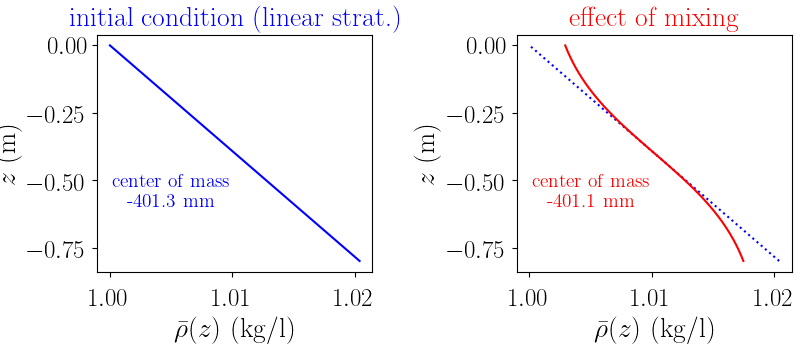
\includegraphics[width=\figwidth]{tmp/fig_scheme_mixing}
\caption{Scheme representing the effect of mixing on the density profile and
the center of mass.}%
\label{fig:average:mixing}
\end{figure}


\subsection{Overview of the experiment}

The experimental setup, installed in the large Coriolis platform, is presented
in figure~\ref{fig:exp}: a tank with a rectangle base of 9$\times$6~m$^2$ area
is filled with an approximately linear salt stratification of $81$~cm depth.

The flow is generated with an oscillating comb. Two different combs were used:
the first one in made of 6 vertical cylinders of $25$~cm diameter attached to a
carriage with a mesh of $M=75$~cm, and for the second one, there are 4
cylinders of $50$~cm diameter with a mesh of $M=1.5$~m. We impose on the
carriage the following periodic motion of period $T$ (see figure~\ref{fig:exp}
for a chronogram of its position $x_c$): it accelerates with a constant
acceleration over 25~cm to a velocity $U_c$, travels at the uniform speed a
distance of 650~cm and decelerates with a constant deceleration over 25~cm. It
them comes back to its initial position with the opposite movement and
immediately restarts this cycle. In the following, we use cartesian coordinates
with the origin centered with respect to the vertical walls and at the bottom
of the tank. The vertical coordinate is given by $z$ and the horizontal
coordinate along the direction of displacement of the carriage by $x$ such that
$(x,y,z)$ form right handed coordinates.

We use in this study results from two different experimental campains, carried
out in 2016 and 2017. In the following, the two sets of experiments are denoted
as MILESTONE 2016 (``M16") and MILESTONE 2017 (``M17"). The M16 campain has
already been described in \cite{campagne2016}. 
The two experimental setups are
nearly identical. They differ mainly on the precise locations of the density
and temperature probes and on the number and the precise locations of the
cameras used for Particle Image Velocity (PIV). For the second set of
experiments (M17), the carriage is accelerated over 0.5 cm and travels at
constant speed over 5~m. The constant speed is varied from 1 cm/s up to 24
cm/s.

\begin{figure}[htp!]
\centering
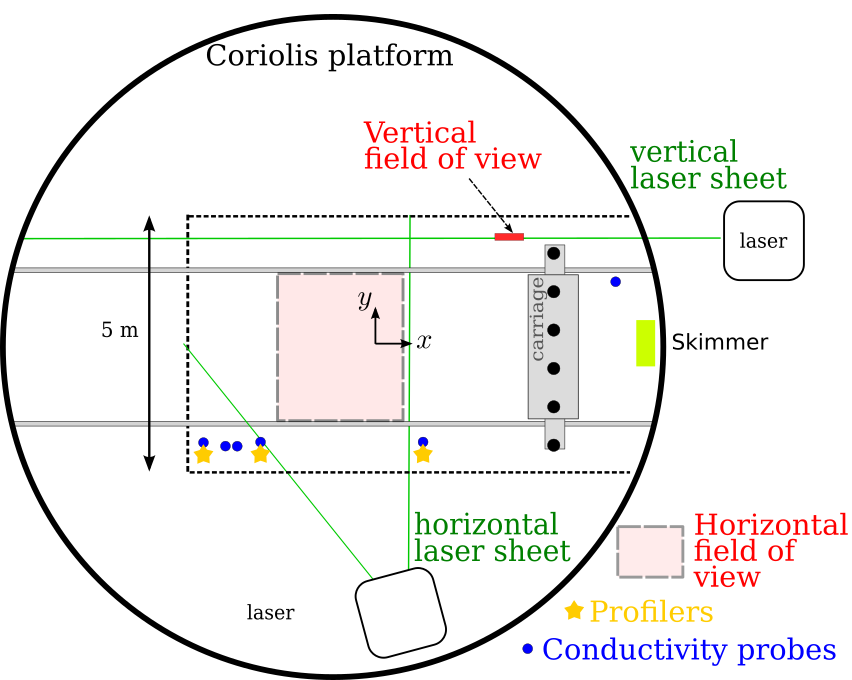
\includegraphics[width=80mm]{../figs/scheme_milestone17}\\[5mm]
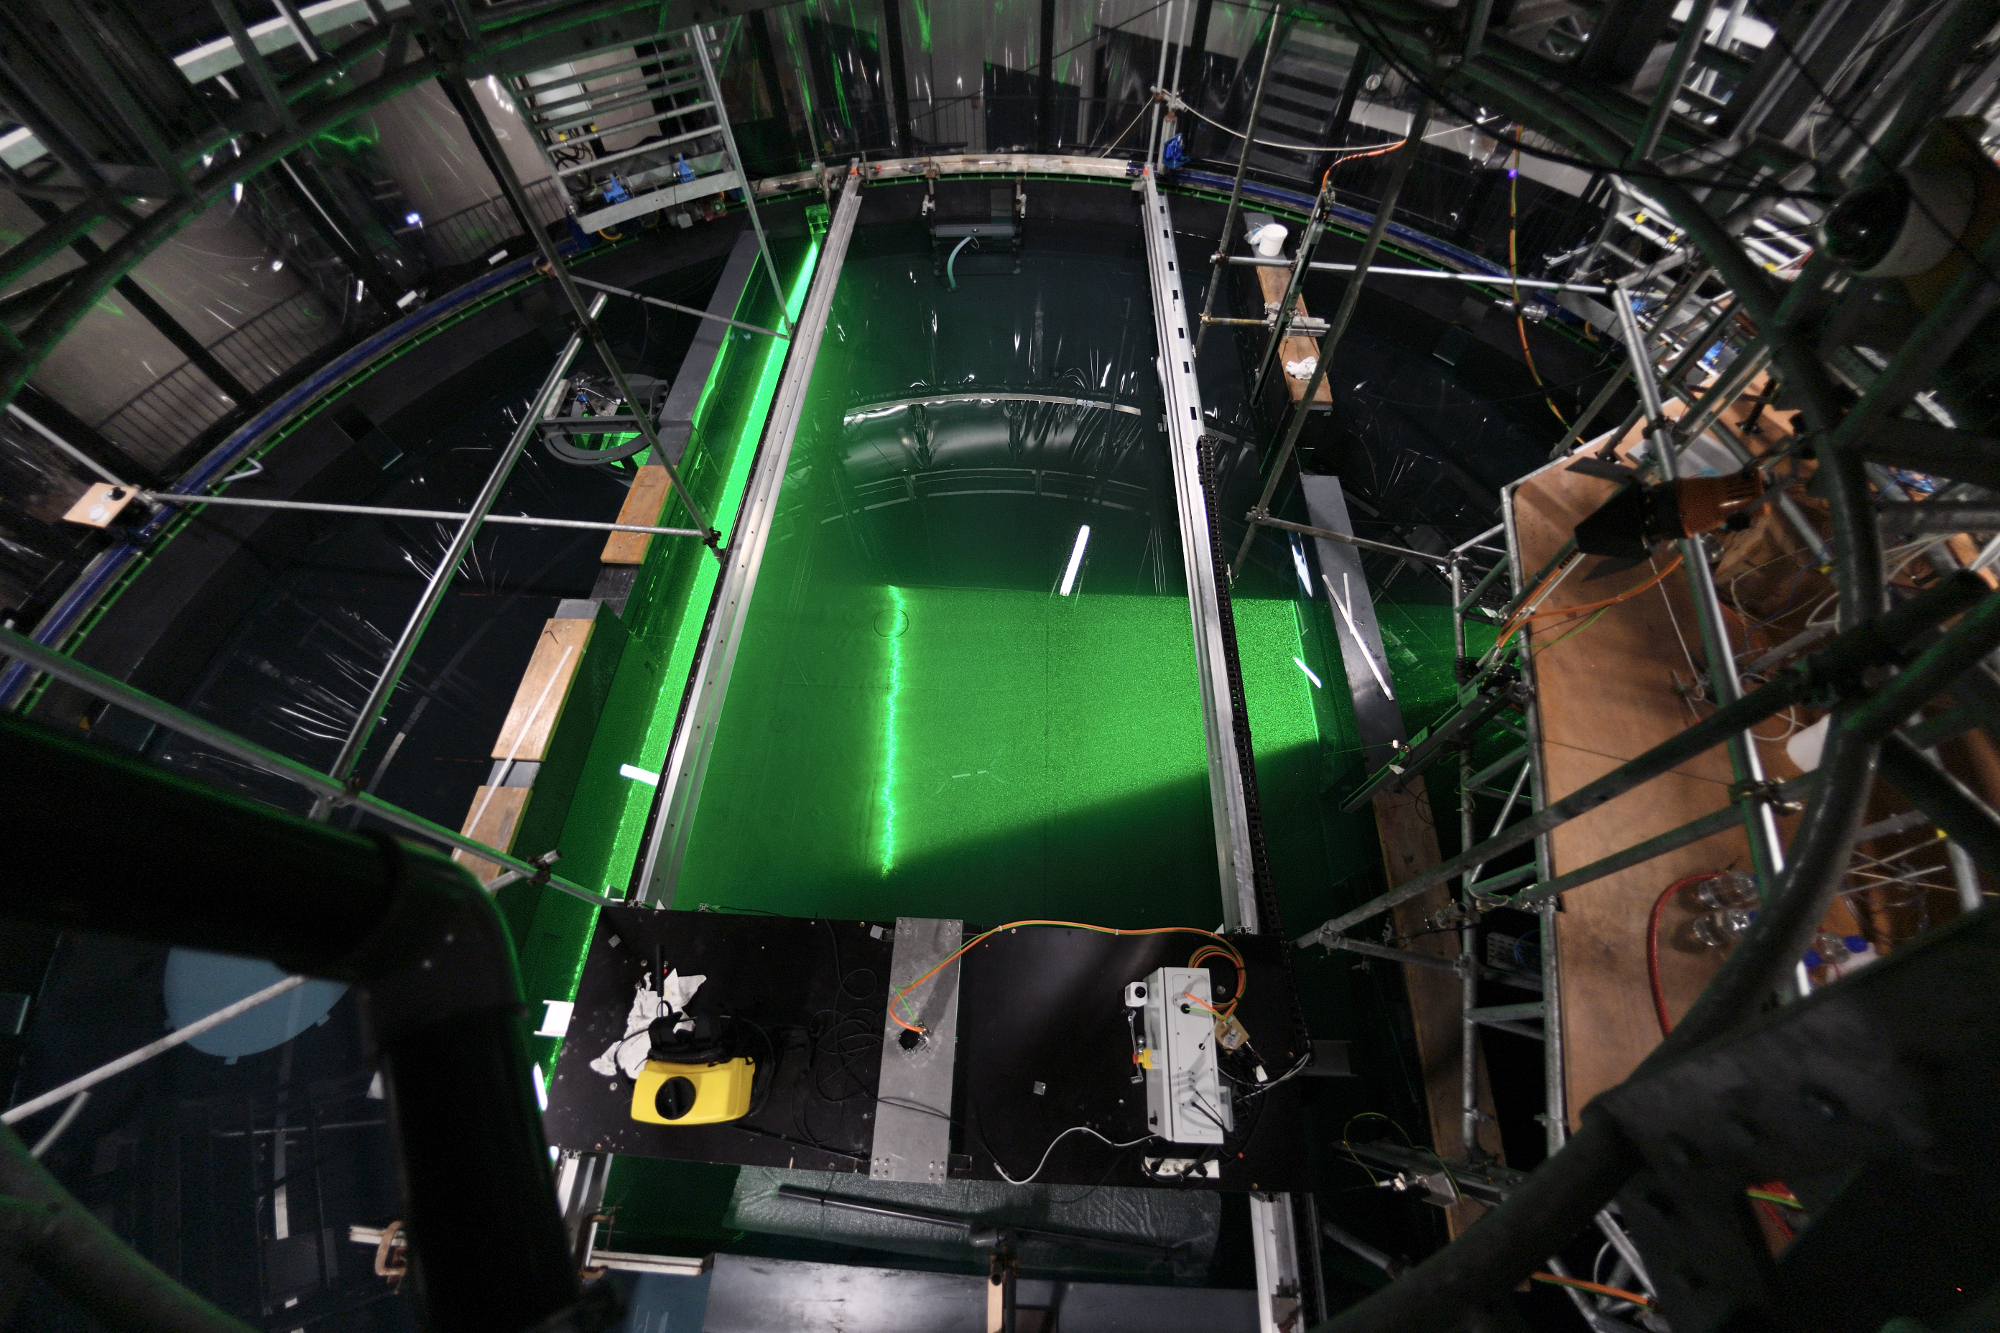
\includegraphics[width=80mm]{../figs/milestone17_top}
% 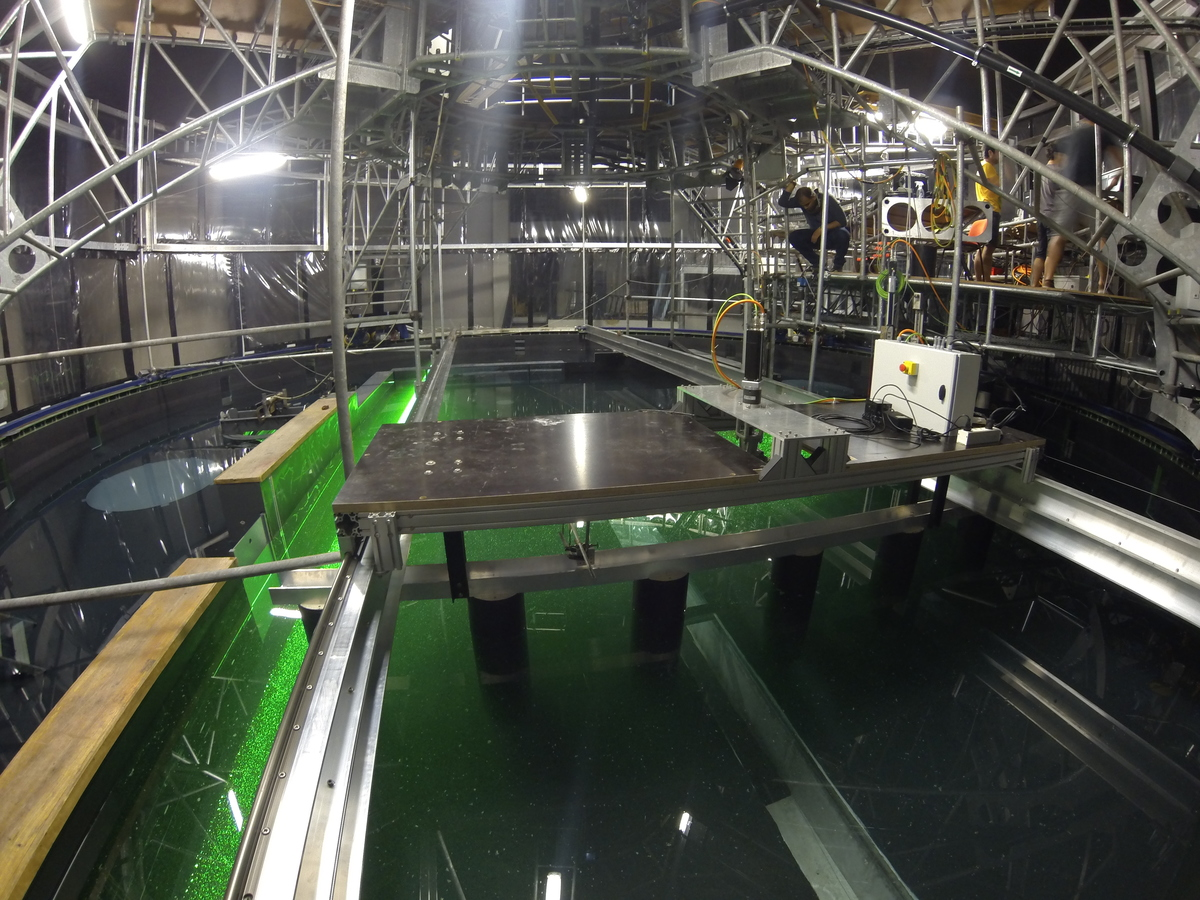
\includegraphics[width=\figwidth]{../figs/real_setup_milestone}
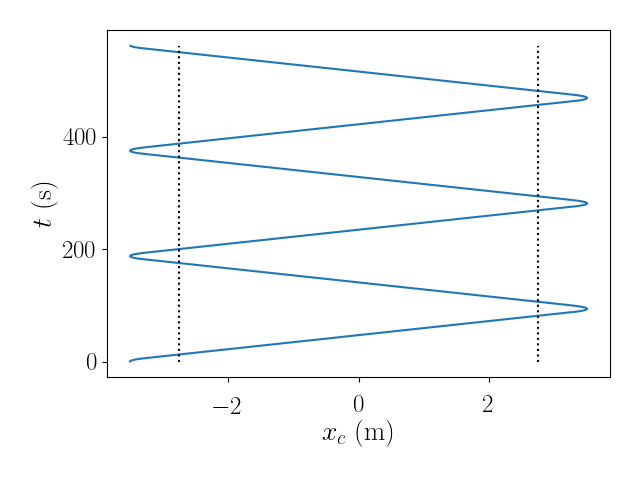
\includegraphics[width=80mm]{tmp/fig_movement_carriage}

\caption{Top: scheme of the experimental setup for the MILESTONE 2017
experiments (see text for description). Center: photography of the experiment.
Bottom: chronogram of the position of the carriage $x_c(t)$.}%
\label{fig:exp}
\end{figure}

Density is measured with temperature and conductivity probes which are either
static (to measure the density at the top and the bottom of the tank), attached
to the carriage or attached to traverses to obtained density profiles.

To be able to accurately measure the mixing, the slow experiments are very long
($\sim$ 5 hours, i.e. more than 10 periods of oscillation of the carriage). In
contrast, the mixing is much faster for the larger velocity so it is difficult
to maintain the forcing during more than 2 or 3 periods of oscillation and
therefore to get a lot of statistics.

The velocity is measured by Particle Image Velocity (PIV). While we used 5
cameras in the M16 campain, for M17 experiments, we use only 3 cameras. One is
dedicated to record images for horizontal scanning PIV with up to 16 vertical
levels. The two other cameras are used for stereoscopic vertical 2D PIV.


\begin{table}
\centering
\begin{tabular}{lcccccc}
    \toprule
    &   $Uc$ &  $D_c$ &  $N$  &  $F_{hc}$ &  $Re_c$ &   $\R_c$  \\
    & (cm/s) &   (cm) &(rad/s)&           &         &           \\
    \midrule

 M16-18 &   2 &  25 &  0.76 &  0.100 &   5000 &     50 \\
 M16-21 &   8 &  25 &  0.76 &  0.400 &  20000 &   3200 \\
 M16-22 &   4 &  25 &  0.77 &  0.200 &  10000 &    400 \\
 M16-24 &  16 &  25 &  0.75 &  0.800 &  40000 &  25600 \\
 M16-32 &   2 &  25 &  0.58 &  0.143 &   5000 &    102 \\
 M16-33 &   2 &  25 &  0.58 &  0.143 &   5000 &    102 \\
 M16-34 &   4 &  25 &  0.57 &  0.286 &  10000 &    816 \\
 M16-35 &   4 &  25 &  0.57 &  0.286 &  10000 &    816 \\
 M16-64 &   2 &  25 &  0.74 &  0.100 &   5000 &     50 \\
 M16-65 &   2 &  25 &  0.74 &  0.100 &   5000 &     50 \\
 M16-66 &   4 &  25 &  0.75 &  0.200 &  10000 &    400 \\
 M16-68 &   6 &  25 &  0.76 &  0.300 &  15000 &   1350 \\
 M16-69 &   6 &  25 &  0.74 &  0.300 &  15000 &   1350 \\
 M16-70 &   8 &  25 &  0.76 &  0.400 &  20000 &   3200 \\
 M16-71 &  12 &  25 &  0.70 &  0.600 &  30000 &  10800 \\
 M16-72 &  16 &  25 &  0.68 &  0.800 &  40000 &  25600 \\
 M16-73 &  16 &  25 &  0.56 &  0.800 &  40000 &  25600 \\
 M17-11 &  16 &  25 &  0.55 &  1.164 &  40000 &  54162 \\
 M17-17 &   4 &  50 &  0.55 &  0.145 &  20000 &    423 \\
 M17-18 &   8 &  50 &  0.55 &  0.291 &  40000 &   3385 \\
 M17-19 &   2 &  50 &  0.55 &  0.073 &  10000 &     53 \\
 M17-20 &   2 &  50 &  0.55 &  0.073 &  10000 &     53 \\
 M17-21 &  12 &  50 &  0.55 &  0.436 &  60000 &  11425 \\
 M17-22 &  12 &  50 &  0.55 &  0.436 &  60000 &  11425 \\
 M17-23 &  16 &  50 &  0.55 &  0.582 &  80000 &  27081 \\
 M17-34 &   2 &  25 &  0.55 &  0.145 &   5000 &    106 \\
 M17-35 &   1 &  25 &  0.55 &  0.073 &   2500 &     13 \\
 M17-36 &   4 &  25 &  0.55 &  0.291 &  10000 &    846 \\
 M17-37 &   8 &  25 &  0.55 &  0.582 &  20000 &   6770 \\
 M17-39 &  12 &  25 &  0.55 &  0.873 &  30000 &  22850 \\
 M17-40 &  12 &  25 &  0.55 &  0.873 &  30000 &  22850 \\
 M17-41 &  16 &  25 &  0.55 &  1.164 &  40000 &  54162 \\
 M17-42 &  24 &  25 &  0.55 &  1.745 &  60000 &  182797 \\
 M17-43 &  24 &  25 &  0.55 &  1.745 &  60000 &  182797 \\
 \bottomrule
\end{tabular}
\caption{\label{table:exp} Experiments used for this study.}
\end{table}


\subsection{Open-data and open-source}

% Ashwin can write this part...

\input{paper_06_milestone/1st/sec_open_science.latex}
% An interesting particularity of the MILESTONE experiment is to be based on
% open-source method and to provide open datasets and open-source packages to
% load and analyze them.
%
% Two open-source Python packages called FluidLab and FluidCoriolis
% \cite{fluiddyn} were developed for these experiments and used to control most
% of the objects during the experiments.
%
% For example the movement of the carriage and of the probes are controlled with
% a graphical application and Python scripts provided by fluidlab and
% FluidCoriolis. Horizontal scanning PIV is also made possible by controling the
% rotating mirror and the triggers of the camera by functions provided in
% fluidlab. This allows anyone to perform horizontal scanning PIV with a good
% camera (here a PCO Edge), a rotating mirror and a quite cheap acquisition board
% (T7 LabJack) to trigger the camera.
%
% FluidLab is a generic API for orchestrating laboratory experiments. The
% software leverages the object-oriented programming features in Python to model
% real life instrumentation. An experiment in the simplest level can be thought
% of as a network of interconnected instruments awaiting commands and also
% sending and receiving data.
%
% The computation of PIV fields is performed on the cluster of the LEGI with an
% open-source Python package called fluidimage
%
% Data processing and data opening with FluidCoriolis.


\section{Results}

\subsubsection{Estimating the kinetic energy dissipation rate $\eps_K$}

As already stated, we have not been able to measure the local energy
dissipation. \cite{PraudFinchamSommeria2005} used 3D PIV to compute some terms
of the local kinetic dissipation from velocity fields but only for very slow
flows, corresponding to very small buoyancy Reynolds number. However, when the
velocity is increased, the flow becomes more turbulent and the Kolmogorov
length scale decreases so that it becomes much more difficult to compute
accurately the velocity gradient from PIV velocity field.

Therefore, we are forced to estimate the kinetic energy dissipation rate from
the decay of the kinetic energy, which is a large-scale quantity. By averaging
the energy computed from several horizontal PIV fields (different vertical
levels and periods of the carriage), we can evaluate the averaged time
evolution of the kinetic energy after one stroke and finally the averaged
kinetic energy dissipation.

\begin{figure}[htp!]
\centering
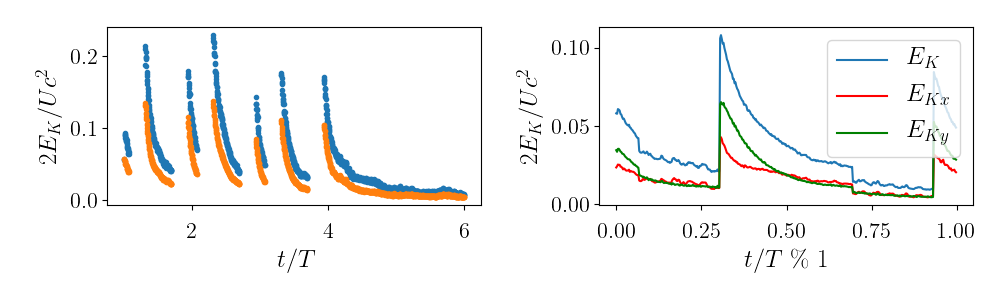
\includegraphics[width=0.5\textwidth]{tmp/fig_energy_vs_time}

\caption{Kinetic energy decay for experiment M16-73.}%
\label{fig:energy:vs:time}

\end{figure}

Figure~\ref{fig:energy:vs:time} shows the time evolution of the mean kinetic
energy in the region scanned by the horizontal PIV. For this experiment
(M16-73), the carriage oscillates during 4 periods and is then stopped.

\begin{figure}[htp!]
\centering
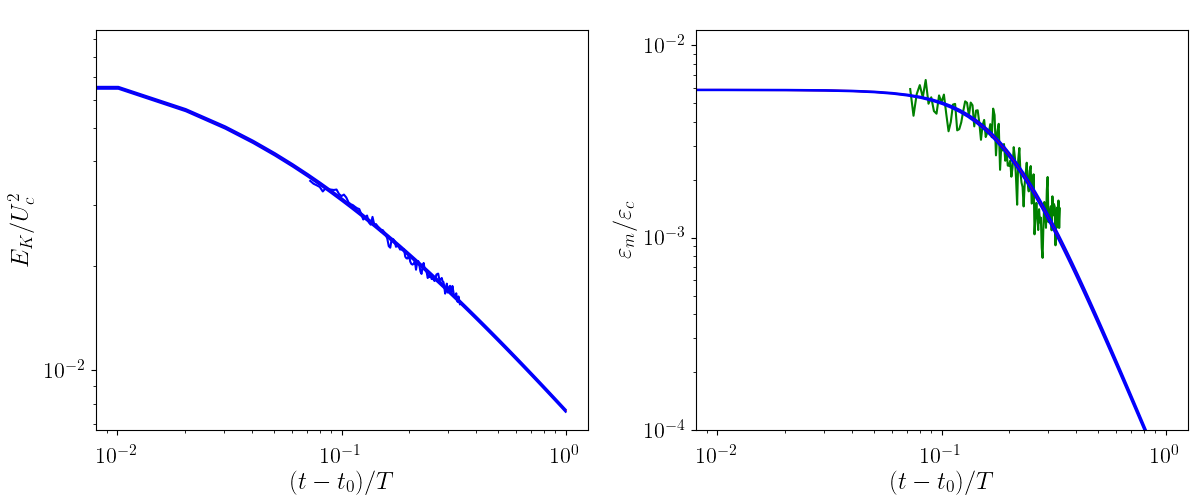
\includegraphics[width=80mm]{tmp/fig_fit_EK}

\caption{Fits of the kinetic energy decay for M16-73 (same as in
figure~\ref{fig:energy:vs:time}). The time derivatives of the kinetic energy in
(b) are normalized by $\eps_c = U_c^3 / D_c$.}%
\label{fig:fit:EK}

\end{figure}

Figure~\ref{fig:fit:EK}(a) shows the space and phase averaged kinetic energy as
a function of $(t - t_0)/T$ and a fit of the data $a / (1 + t^\alpha)/\beta$.
Figure~\ref{fig:fit:EK}(b) presents the time derivative of the kinetic energy
and the same quantity obtained from the fit of the kinetic energy. We finally
compute by averaging over time for $t < 0.5 T$, $\eps_m= \mean{d_t E_{Kh}}$, an
estimation of the kinetic energy dissipation averaged over few turnover times
after the strokes.

\begin{figure}[htp!]
\centering
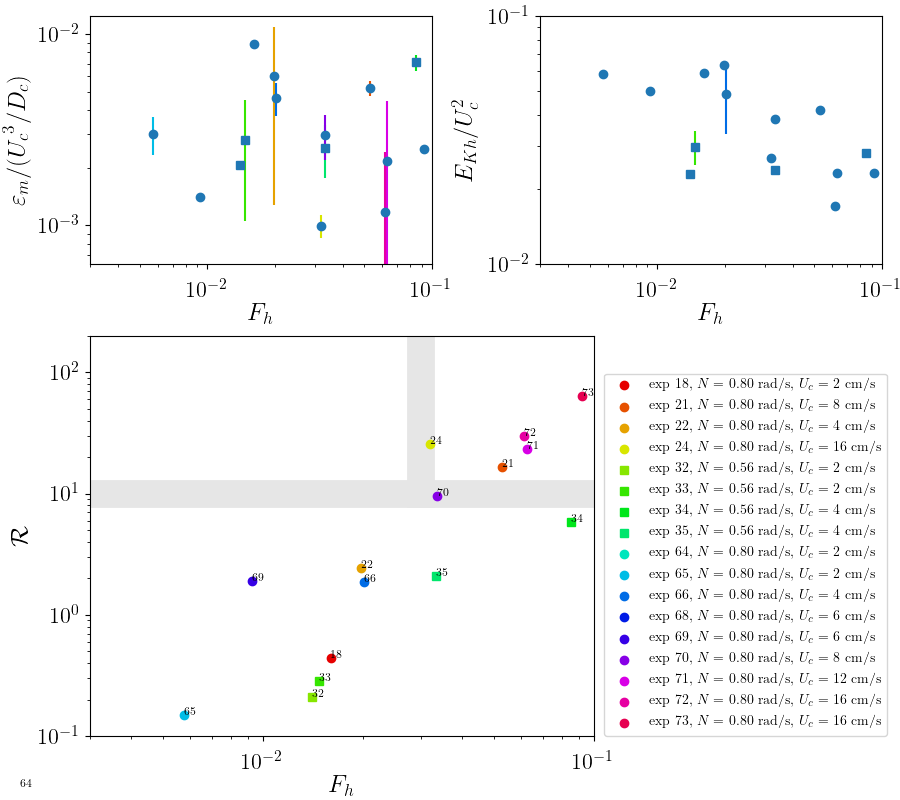
\includegraphics[width=\figwidth]{tmp/fig_R_vs_Fh}%

\caption{Evaluation of the buoyancy Reynolds number $\R$ and the horizontal
Froude number $F_h$ from the horizontal kinetic energy $E_{Kh}$ and its decay
$\eps_m = \mean{d_t E_{Kh}}$ for the M16 experiments.}%
\label{fig:RvsFh}

\end{figure}

Together with the mean Brunt-V\"ais\"al\"a frequency computed from the density
profiles, we are able to estimate the values of $\R$ and $F_h$ for each
experiment. The values of $E_{Kh}$, $\eps_m$, $\R$ and $F_h$ are plotted in
figure~\ref{fig:RvsFh}. Horizontal and vertical grey bars have been added to
delimit the 3 regimes of stratified flows, namely strongly stratified
turbulence ($F_h < 0.03$), weakly stratified turbulence ($F_h > 0.03$), and
low-$\R$ stratified flows (affected by dissipation at large horizontal scale).

We see that with these estimations, none of the M16 experiments is really in
the strongly stratified turbulence regime. However, some experiments are close to
the thresholds and we have to stress that these estimates of $E_{Kh}$ and
$\eps_K$ are computed from a time average for $t < 0.5 T$.

\begin{figure}[htp!]
\centering
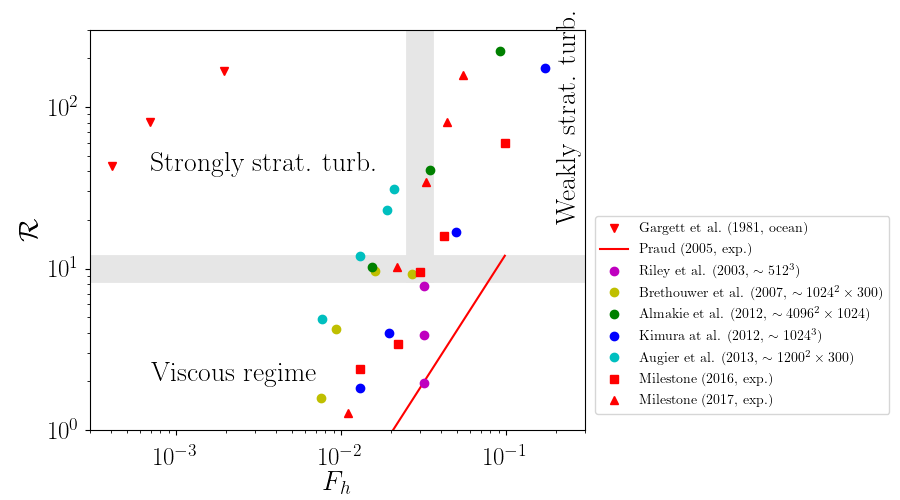
\includegraphics[width=\figwidth]{tmp/fig_R_vs_Fh_other_studies_with_milestone17}%

\caption{Buoyancy Reynolds number $\R$ versus horizontal Froude number $F_h$
for few M16 and M17 experiments and for other experimental and numerical
studies of stratified turbulence.}%
\label{fig:RvsFh:other}

\end{figure}

In figure~\ref{fig:RvsFh:other}, we compare the typical values of the
non-dimensional numbers reached in these experiments with values evaluated for
other studies.


\subsubsection{Evaluation of the mixing coefficient}

Similarly as for the kinetic energy dissipation, we have not been able to
measure the different terms of the density gradient, which are needed to
compute the local available potential energy dissipation. In order to estimate
the mixing, we measure the rate of increase of the average background potential
energy.

\begin{figure}[htp!]
\centering
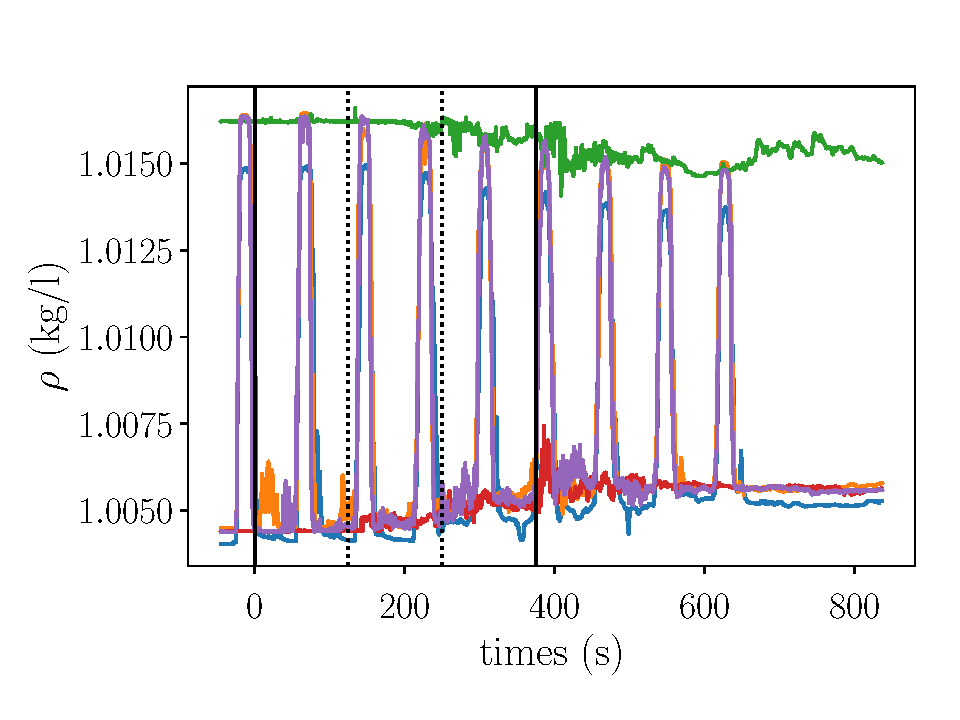
\includegraphics[width=0.7\textwidth]{tmp/fig_rho_vs_time}\\
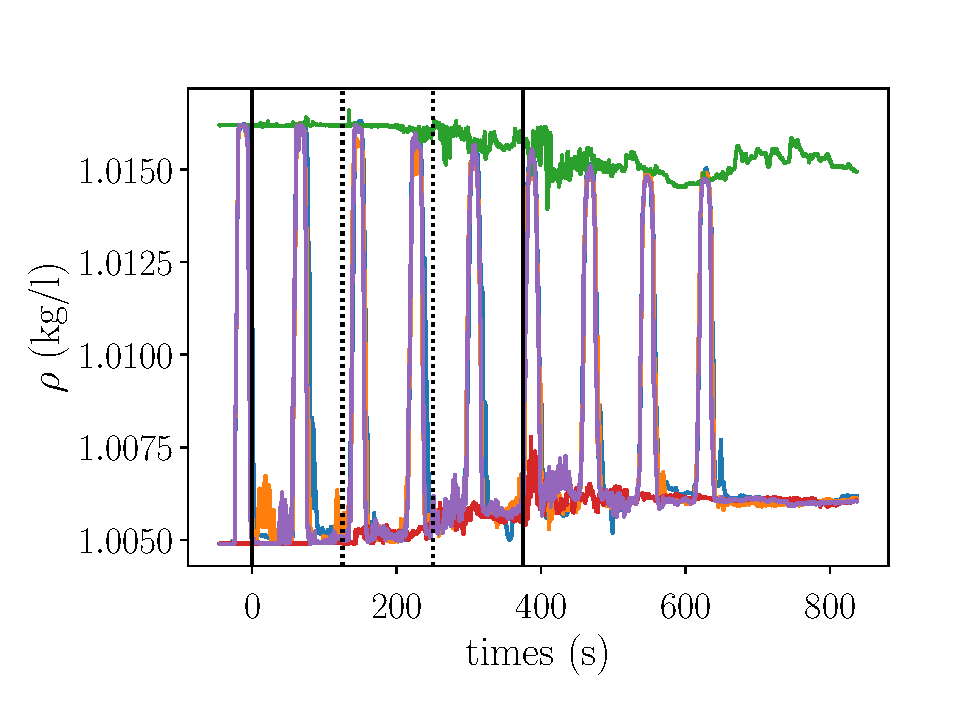
\includegraphics[width=0.7\textwidth]{tmp/fig_rho_vs_time_corrected}

\caption{Density signals measured by the 5 density probes for experiment M17-21
corresponding to $D = 0.5$~m, $N=0.55$~rad/s and $U=12$~cm/s. Three probes are
attached to vertical profilers. The two other fixed probes are at the top and
at the bottom, respectively. (a) raw signals and (b) signals corrected to
compensate a derive of the probes.
}%
\label{fig:rho:vs:time}

\end{figure}

To evaluate this quantity, we need a good measurement of the evolution of the
space-average density profile. Figure~\ref{fig:rho:vs:time}(a) shows the
density signals of 5 probes. Three of these probes are attached to traverses
and the two others are attached at the top and the bottom of the tank. We see
that some probes do not give accurate measurements of the density, so we
correct these measurements with the more precise probes as show in
figure~\ref{fig:rho:vs:time}(b).

\begin{figure}[htp!]
\centering
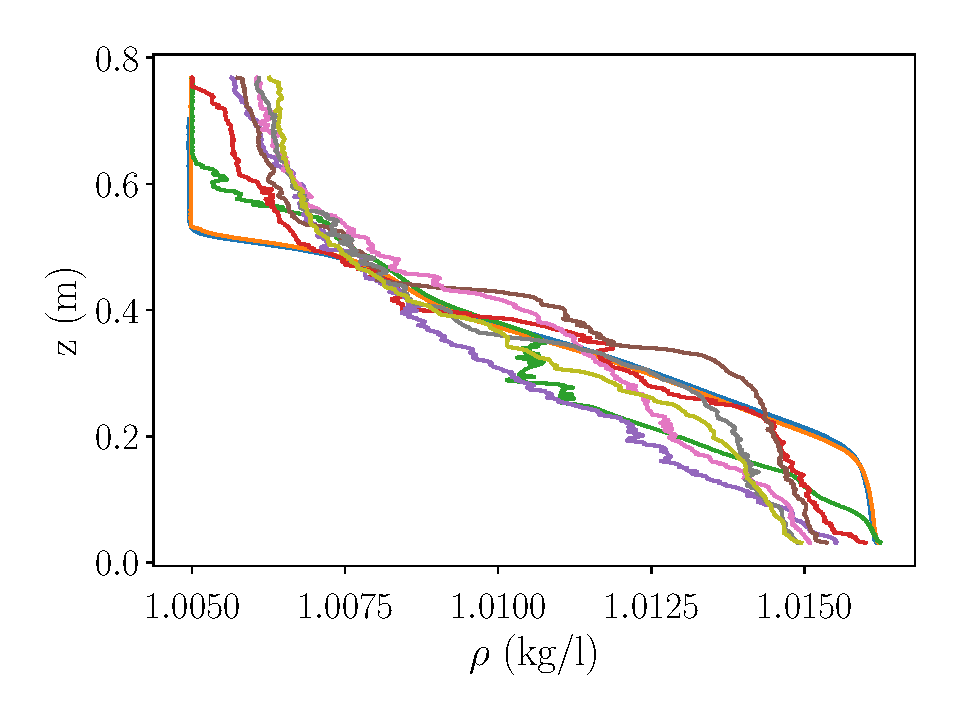
\includegraphics[width=0.7\figwidth]{tmp/fig_profiles_mixing}
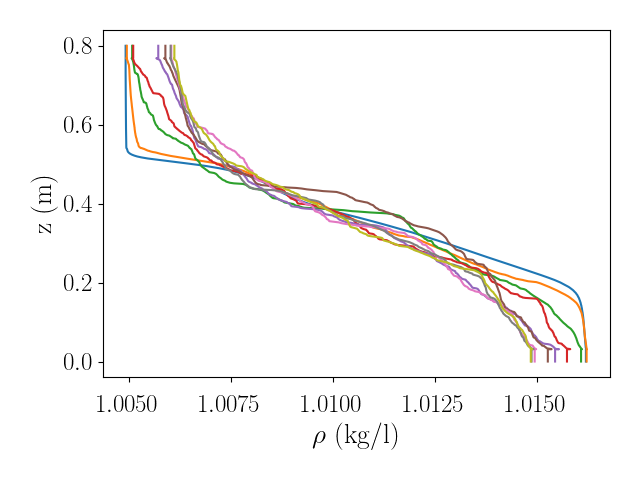
\includegraphics[width=0.7\figwidth]{tmp/fig_profiles_probe_averaged}

\caption{Evolution of the density profiles for experiment M17-21 corresponding
to $D = 0.5$~m, $N=0.55$~rad/s and $U=12$~cm/s.}%
\label{fig:profiles:mixing}

\end{figure}

The space-averaged density profiles computed from these measurements are
displayed in figure~\ref{fig:profiles:mixing}(a). The shape of these profiles
at the top and the bottom is especially important to compute the background
potential energy. However, the probes attached to profilers cannot measure the
density very close to the top and bottom boundaries. The profiles are extended
with values computed from their extrema values as presented in
figure~\ref{fig:profiles:mixing}(b).

\begin{figure}[htp!]
\centering
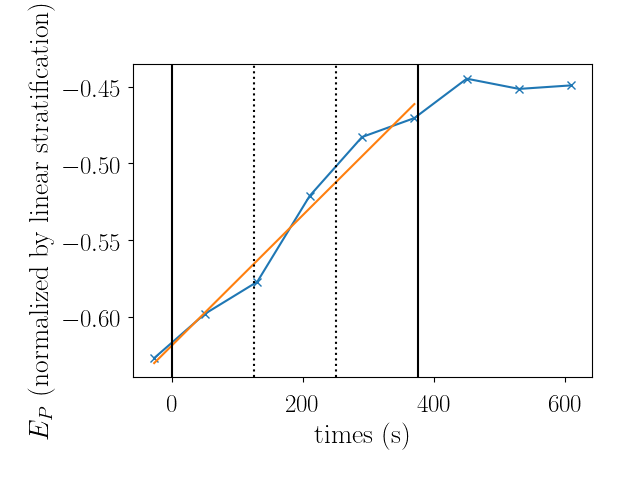
\includegraphics[width=0.7\figwidth]{tmp/fig_energy_pot_vs_time}

\caption{Evolution of the normalized potential energy for experiment M17-21
corresponding to $D = 0.5$~m, $N=0.55$~rad/s and $U=12$~cm/s.}%
\label{fig:energy:pot:vs:time}

\end{figure}

The evolution of the background potential energy is shown in
figure~\ref{fig:energy:pot:vs:time} for the same experiment M17-21. The value
-1 would correspond to a linear stratification with the same initial
Brunt-V\"ais\"al\"a frequency. Since the profiles at the beginning of the
experiment are already eroded, the initial normalized potential energy is
slighly smaller than -0.6. We see that it increases approximately linearly with
time while the fluid is stirred and stabilize at a constant value after the
stop of the carriage. From this curve, we can evaluate the mean rate of
increasement of the average background potential energy $\eps_P$ during an
experiment.


\begin{figure}[htp!]
\centering
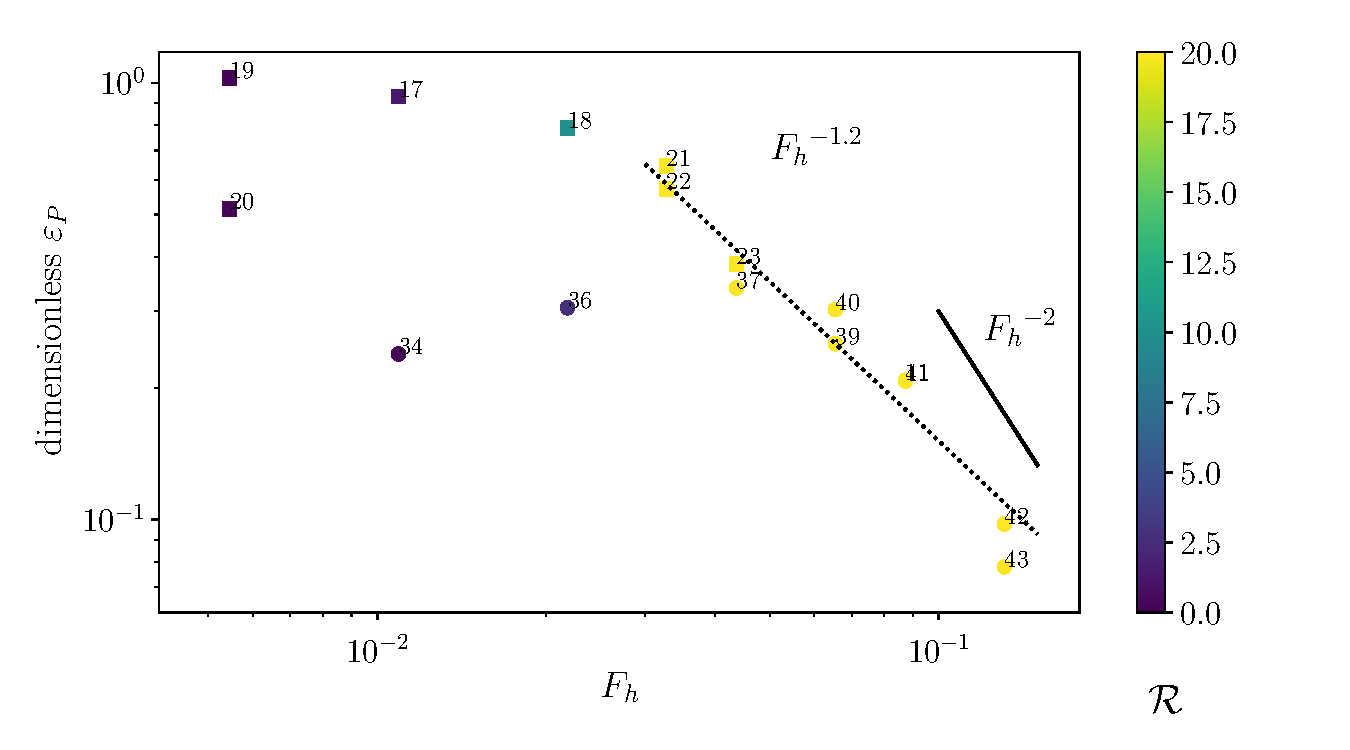
\includegraphics[width=\figwidth]{tmp/fig_dt_pot_energy}

\caption{Normalized mixing coefficient $\eps_P / (3\times10^{-3} {U_c}^3/D_c)$
for some MILESTONE 17 experiments.}%
\label{fig:dt:pot:energy}

\end{figure}

This quantity normalized by an estimation of the dissipation of kinetic energy
$3\times10^{-3} {U_c}^3/D_c$ (see figure~\ref{fig:RvsFh}) is plotted as a
function of the Froude number in figure~\ref{fig:dt:pot:energy}. This quantity
is approximately proportional to the mixing coefficient $\Gamma$. The colors
represent the buoyancy Reynolds number such that the yellow points correspond
to $\R > 15$. We see that the yellow points fall on a same curve, while there
are more variations for smaller values of buoyancy Reynolds number. The yellow
points are more consistent with a ${F_h}^{-1}$ than with the ${F_h}^{-2}$
scaling law observed and predicted with \cite{Maffioli2016}.

\section{Conclusions}

???
